\documentclass[conference]{sig-alternate-05-2015}
\usepackage{color, xcolor, float, lscape, enumerate, graphicx, url, tabularx, multirow, xspace, hyperref}%times
\usepackage[font=bf, skip=0pt]{caption}
\usepackage[shortlabels,inline]{enumitem}
\usepackage{mathtools}
%\usepackage{titlesec}
\usepackage[english]{babel}
\DeclareMathOperator*{\argmax}{arg\,max}
\DeclarePairedDelimiter\abs{\lvert}{\rvert}%
\DeclarePairedDelimiter\norm{\lVert}{\rVert}%

\graphicspath{ {./images/} }

\hypersetup{
  colorlinks,
  citecolor=blue,
  linkcolor=red,
  urlcolor=black}
\newcommand{\note}[1]{{\textcolor{blue}{[#1]}}}
\newcommand{\fixme}[1]{{\textcolor{red}{#1}}}
\newcommand{\citeme}{{\textcolor{red}{[?]}}\xspace}
\newcommand{\todo}[1]{{\textcolor{red}{[#1]}}}
\newcommand{\BfPara}[1]{{\noindent\bf#1.}\xspace}
\newcommand{\vi}{\vspace{5mm}}
\newcommand{\etal}{{\em et al.}\xspace}
\newcommand{\eg}{{\em e.g.,}\xspace}
\newcommand{\ie}{{\em i.e.,}\xspace}
\newcommand{\etc}{{\em etc}\xspace}



\usepackage{fancyvrb}
\usepackage{verbatim}
\begin{document}



\title{Cyber-Bullying Detection and Classification System}



\author{
  Marc Mailloux\\ marcmailloux@knights.ucf.edu
  \and Rolando Nieves\\ rolando.j.nieves@knights.ucf.edu
  \and Maxim Shelopugin\\ maxim.shelopugin@knights.ucf.edu
}

\maketitle


\section{Introduction}\label{sec:introduction}
Among all the forms of bullying and harassment recognized today, bullying via
platforms hosted on the Internet has proliferated at an alarming rate. The rate
of proliferation has been concerning enough to motivate the United States
Centers for Disease Control and Prevention (CSC) to acquire and report data
regarding ``electronic'' bullying (or, as it is more commonly known,
``cyber-bullying'' via its biennial Youth Risk Behavior Surveillance System
(YRBSS) \cite{CBRC_facts2018}.

Collection of data from cyber-bullying victims has helped immensely as it
pertains to awareness and prevention. It should be possible to further improve
in both areas if data collection overcomes the limitation of the
``a posteriori'' nature of current methods (i.e., prevention methods derived
from data voluntarily disclosed by victims after harassment has occurred). An
automated system capable of examining electronic communication traffic,
identifying and classifying any traffic that could be considered as bullying,
could lead to solutions that can either filter out any offensive content
automatically, or significantly shorten the response time to an incident,
possibly preventing the more dire secondary effects of cyber-bullying.

The report content as follows will begin with a formal statement of the problem
the authors attempt to address. Following will be a short survey of works that
are related to the system documented in this paper. Then, a discussion of the
system's methodology will dive into the inner workings, detailing how the system
attempts to solve the aforementioned problem, as well as detailing how the
system's performance will be profiled. The following sections covers
briefly the risks identified and/or realized during implementation, and how, if
at all, they were mitigated. After the discussion on risks, the system's
performance is documented by following the system profiling plan detailed in
the section covering the system's methodology. The system performance profile is
then followed by a short discussion regarding insights gleaned from the system
performance profile. After the system performance discussion, the work breakdown
and delegation scheme applied during system implementation will be covered.
Finally, the paper will conclude with short statements regarding the overall
investigation, including possibilities for future enhancements to the work.

\section{Problem Statement}\label{sec:problem_statement}

The methods presented in this paper document the implementation of a
proof-of-concept system that is able to accept short messages in plain text,
and classify these messages, identifying those with content that could be
considered as cyber-bullying. Leveraging technological advances in Natural
Language Processing, along with algorithms borrowed from the areas of Artificial
Intelligence and Machine Learning, the system will be trained to recognize and
classify cyber-bullying traffic. The classification will go beyond simply
identifying bullying traffic, but will also categorize the bullying into three
(3) distinct classes:
\begin{description}
    \item[Cultural Harassment] Offensive content primarily focusing on the
    victim's race or religious beliefs.
    \item[Sexual Harassment] Amplification of stereotypical behavior for a given
    gender, or gender identification.
    \item[Personal Attacks] Ridicule based on a victim's outward-visible
    attributes, such as appearance, mannerisms, or intelligence.
\end{description}

\section{Related Work}\label{sec:related}

There has been much research done around this topic, as evidenced by the body of
work on display on the Cyber-Bullying Research Center research summary page
\cite{CBRC_research2018}. Approaches employed to date include relatively
simple Bayes type classifiers, as well as more complex deep learning systems
(Sweta Agrawal et. al. \cite{agrawal2018deep}). One existing implementation that
serves as an excellent exemplar to this proof-of-concept implementation is the
\textit{Anti Bully} project by Michelle Li \cite{Li2016}. The work documented
in this report differs from \textit{Anti Bully} in two important ways:

\begin{itemize}
  \item The implementation documented in this paper does not rely solely on
  Na\"{i}ve Bayes classification algorithms the way \textit{Anti Bully} does.
  \item The system will be able to further refine the binary
  classification done in \textit{Anti Bully} (which only identifies traffic as
  \textbf{bullying} or \textbf{not bullying}) by categorizing bullying traffic
  among one of the classes listed in Section \ref{sec:design}.
\end{itemize}

The \textit{Anti Bully} system code base does include a good data set which can
be used in the proof-of-concept documented in this paper, albeit with some
modifications (see Section \ref{subsec:eval_dataset}).

A library that has proven invaluable in the proof-of-concept implementation
documented in this paper is the \textit{Natural Language Toolkit (NLTK)}
(Bird et. al. \cite{bird2009natural}). The primary \textit{NLTK} features
leveraged in this proof-of-concept include:
\begin{itemize}
  \item Split content into sentences and words
  \item Filter out ``Stop Words'' (e.g., ``the,'' ``a,'', ``is'')
  \item ``Stemming'' (i.e., reducing words to their root)
\end{itemize}

The tutorial by Jason Brownlee titled ``How to Clean Text for Machine Learning
with Python'' \cite{brownlee-2017} was instrumental in learning how to
effectively use these \textit{NLTK} features. Indeed, the proof-of-concept
implementation documented in this paper incorporates code snippets offered in
said tutorial.

Another library that has proven very useful in this proof-of-concept
implementation, especially in the area of numerical processing, is the
\textit{TensorFlow} library produced by Google, Inc.
\cite{tensorflow2015-whitepaper}. The primary list of \textit{TensorFlow}
features used in this proof-of-concept are:
\begin{itemize}
  \item Ready-made constructs for:
  \begin{itemize}
    \item Artificial Neuron Networks (ANN)
    \item Linear and Radial Basis Function-based Support Vector Machines (SVM)
  \end{itemize}
  \item High performance parallel computing leveraging Graphical Processing
  Unit (GPU) capabilities
\end{itemize}

The design decision (as documented in Section \ref{sec:design}) regarding the
use of Comma Separated Value (CSV)-formatted files as primary input/output led
to the inclusion of the Pandas data processing library
\cite{mckinney-proc-scipy-2010}.

Finally, serving as the foundation for nearly all of these external libraries,
is the \textit{NumPy} numerical computation library \cite{oliphant2006guide}.

\section{Methodology}\label{sec:design}

The system, at its core, is very similar to classification systems
common in the areas of Artificial Intelligence and Machine Learning. The system
combines a classifying apparatus based on machine learning algorithms with a
natural language vector representation mechanism.

The inner workings of the system can be described as an information flow,
ultimately leading to output artifacts containing the data included in this
report. The information flows through the following set of processes (some of
which are further described in later subsections, as referenced in each list
item):
\begin{enumerate}
  \item \textbf{Pre-processing:} Accept the original input from the data set and
  prepare the data set text for feature representation (see Section
  \ref{subsec:preprocessing}).
  \item \textbf{Feature Representation:} Accept the processed input and
  transform it into vector-based feature representations (see Section
  \ref{subsec:feature_rep}).
  \item \textbf{Classification and Evaluation:} Train a classifier to predict
  labels for each of the samples in the data set, compare said predictions to
  the actual data set labels, and produce metrics describing the classification
  performance (see Section \ref{subsec:classification}). Three independent
  classifiers are used within this task:
  \begin{itemize}
    \item ANN classification - A three-layer (one input, one hidden, and
    one output) Artificial Neuron Network (ANN).
    \item SVM classification - A Support Vector Machine using a Radial Basis Function (RBF) Kernel and Linear Kernel.
    \item Bayes classification - A Na\"{i}ve Bayes classifier.
  \end{itemize}
  \item \textbf{Statistical Significance:} Determine, via statistical tests,
  which classifier(s) perform better than others (see Section
  \ref{subsec:stat_significance}).
\end{enumerate}

A simple diagram depicting the aforementioned information processing tasks, and
how information flows, is shown in Figure \ref{fig:design}.

\begin{figure}[h]
  \centering
  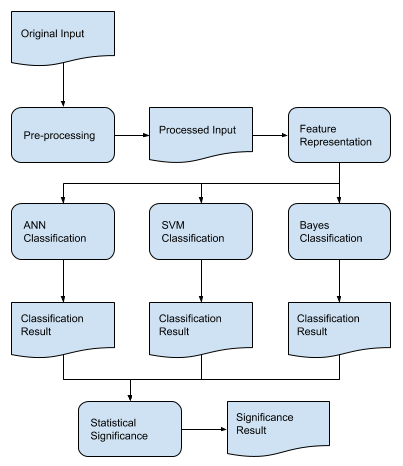
\includegraphics[width=\linewidth]{design.png}
  \caption{Pipeline depicting the high-level design of the Cyber-bullying
  Detection and Classification System that combines both control and data flow
  as the input works its way through the system, eventually leading to the
  outputs that help evaluate the system's performance.}
  \label{fig:design}
\end{figure}

In order to both save required processing time between runs, as well as capture
data that eventually is included in this report, some of these processes produce
artifacts as their resulting product. The complete list of artifacts in the
system follows:

\begin{itemize}
  \item \textbf{Original Input:} The data set as it exists prior to processing.
  \item \textbf{Processed Input:} The data set transformed by the
  \textit{Pre-processing} task (see Section \ref{subsec:processed_input}).
  \item \textbf{Classification Result:} Set of metrics that describe the
  classification performance of its corresponding classifier (see Section
  \ref{subsec:classification_result}).
  \item \textbf{Significance Result:} Statistical analysis derived from the set
  of results produced by all the system's classifiers (see Section
  \ref{subsec:stat_sig_result}).
\end{itemize}

\subsection{Pre-processing}\label{subsec:preprocessing}
The \textit{Pre-processing} process takes the original data set input and
performs the following tasks on it:

\begin{itemize}
  \item Split records and fields in the Comma Separated Values (CSV) input
  \item Replace recognized emoji character combinations with text equivalents
  \item Normalize case in the text within each data set sample
  \item Tokenize the text into words
  \item Filter out punctuation in the sample text
  \item Filter out ``stop words'' in the sample text
  \item ``Stem'' the words present in the sample text
\end{itemize}

\subsection{Processed Input}\label{subsec:processed_input}
As output, \textit{Pre-processing} creates a CSV file with a record for each
original sample, but with the sample's text portion transformed per the
aforementioned tasks.

The motivation behind having the \textit{Pre-processing} flow process produce
its output in the form of an intermediate artifact, as opposed to the more
traditional in-memory data structures, can be summed up in two points:
\begin{itemize}
  \item The time required to pre-process the data set text is not negligible,
  averaging around $15$ minutes for the whole data set.
  \item Write-compile-test cycles on the downstream processes is much more
  efficient with the pre-processor's result readily available.
  \item Downstream processes are not dependent on the \textit{Pre-processing}
  task's run time state.
\end{itemize}

\subsection{Feature Representation}\label{subsec:feature_rep}
The \textit{Feature Representation} process transforms the pre-processed sample
text into vector representations by identifying the unique 3-grams and 4-grams
present in the input, then describing each text sample as a vector expressing
the appearance frequency of these n-grams. N-grams here are the results of process
of splitting the pre-processed chunks of text into the subsets of consecutive
words, where $n$ determines the size of a given subset. The process is able to 
produce vector representations for each text sample based on:
\begin{itemize}
  \item \textbf{3-gram} - The presence count of unique 3-grams in the sample
  \item \textbf{4-gram} - The presence count of unique 4-grams in the sample
  \item \textbf{3 and 4-gram} - The concatenation of the above two results
\end{itemize}

\subsection{Cross-Validation}\label{subsec:cross_validation}
To establish the correctness of hyper-parameters of the model as well as 
evaluate the effectiveness of the system, it is decided to split the data set
into chunks, such that every split generates two disjoint sub-data sets,
which together span the original data set. Such a procedure is known as
\textit{Cross Validation}. The idea behind it is to granulate the data and 
train the models on one part, while testing it on the complimentary part.
Repeating this procedure some $k$ amount of times tests the robustness and 
generalizability of the model, while not posing any need of external data for 
the task.


\subsection{Classification and Evaluation}\label{subsec:classification}
As previously described, the \textit{Classification and Evaluation} process:
\begin{enumerate*}[(1)]
  \item accepts the data set after text samples have been transformed into
  vectors,
  \item uses the data set to train a classifier such that it can predict a label
  for an arbitrary sample,
  \item evaluates its predictions against the known sample labels, and
  \item produces metrics based on said evaluation.
\end{enumerate*}\par

Although the set of classifiers used in the system is quite diverse, they all
share the following design traits:
\begin{itemize}
  \item Since the data set will not contain an explicit training and test set,
  the classifiers all use 5-fold cross-validation to produce classification
  metrics.
  \item The final classification metrics are averaged over each of the
  cross-validation runs.
  \item The classifiers will produce the same set of metrics (see Section
  \ref{subsec:classification_result}).
\end{itemize}

\subsection{ANN Classifier}\label{subsec:ann_classfier}

Artificial Neuron Network (ANN) classifiers attempt to derive discrete
classification labels from input data by extracting and examining latent
features in the input samples. The extraction of features is done by feeding
the vector feature representation of the input samples through a network of
artificial ``neurons'' that, based on model parameters, produce an activation
value based on the provided input. At a very high level, each neuron in the
network is applying a linear transformation on the input, then feeding the
linear transformation through an activation function that eventually produces
the output. Since the input is in the form of vectors, the linear transformation
must be vector-based as well, as show in Equation \ref{eq:ann_linear_xform}. The
final neuron output is the result of this linear transformation, passed through
an activation function. Equation \ref{eq:ann_activation} exemplifies the use of
a \textit{sigmoid} as the activation function, just like the activation function
used in this proof-of-concept implementation.\par

\noindent\hrulefill
\begin{equation}
  \label{eq:ann_linear_xform}
  \textbf{z} = \textbf{W}\textbf{x} + \textbf{b}
\end{equation}

\begin{equation}
  \label{eq:ann_activation}
  \textbf{y} = \sigma(\textbf{z})
\end{equation}

\noindent Where:
\begin{description}
  \item[$\textbf{z}$] - Linear transformation result
  \item[$\textbf{W}$] - Scale factor matrix, usually referred to as weights.
  Part of the model parameter collection.
  \item[$\textbf{b}$] - Linear bias. Part of the model parameter collection.
  \item[$\textbf{y}$] - Activation result; neuron output
  \item[$\sigma$] - Sigmoid activation function 
\end{description}
\noindent\hrulefill

The ANN classifier used in this proof-of-concept was designed to contain a total
of three (3) layers: a input layer, one (1) hidden layer, and an output layer.

The input layer would be wide enough (i.e., contain enough
neurons) to accept each element in the data set feature vectors. Thus, if the
feature vectors can be described as $\textbf{x} \in \mathbb{R}^n$, then the
input layer contains exactly $n$ neurons. 

The hidden layer in this fully-connected ANN was designed to contain a total of
$500$ neurons. In effect, the input $\textbf{x} \in \mathbb{R}^n$ that passes
through this layer is reduced to $\textbf{h} \in \mathbb{R}^{500}$. Given that
the dimensionality of the feature vectors for each tweet in this
proof-of-concept is a minimum of $70,000$, the hidden layer does a very
effective job of extracting the pertinent information from each tweet.

The output layer in the network contains a neuron for each of the classification
labels. For this proof of concept, there are four (4) possible labels, so the
output layer produces values of $\textbf{y} \in \mathbb{R}^4$. The output
layer's result is then transformed using a \textit{classification cross-entropy}
function that eventually turns the output into a probability distribution, with
each distribution element representing each of the classification labels. The
label with the highest probability is deemed to be the network's
\textit{prediction}.

\subsection{Na\"ive Bayes Classifier}\label{subsec:naive_bayes_classifer}

Naive Bayes is a popular in its simplicity probabilistic classifier which is
used across many fields within computer science. In its essence the model learns
the conditional probabilities between the class and a classified instance, with
assumed independence between the blocks of such instance. The label is assigned
based on the greedy rule, such that the class which yields the highest
probability is chosen as an assigned class. A more formal exposition of the
concept is shown in Equation \ref{eq:naive_bayes}.\par

\noindent\hrulefill
\begin{equation}
  \label{eq:naive_bayes}
  \begin{aligned}
    \hat{y}&=\argmax_{j \in J}(P(y_j|X)) \\
    &=\argmax_{j\in J}(P(y_j)P(x_0 | y_j) * P(y_j)P(x_1 | y_j) \ldots P(y_j)P(x_i | y_j) )
  \end{aligned}
\end{equation}

\noindent Where:
\begin{description}
  \item[$\hat{y}$] - a predicted label
  \item[$\argmax$] - a function which returns the argument which yields the
  maximum value of the given function
  \item[$X$] - an input vector which consists of entries ${x_0 ... x_i}$
  \item[$J$] - is a set of all classes
\end{description}
\noindent\hrulefill

As it is seen in the formula, the prediction of a true label is based only on
the prior distribution and the conditional probability of every single element
in the vector to the given label. Such simplicity attracts the attention of
developers from many fields, however the assumption of independence hinders the
algorithm. Although it achieves good performance in some "bag of words" tasks,
it is known to under-perform in sequential data analysis since sequential data
assumes dependence. In this project Gaussian version of Na\"ive Bayes is used,
with pre-determined probabilities of priors (due to the unbalanced data set).
Different architectures were tested, resulting in higher accuracy, but since the
main metric to be optimized is \textit{Recall}, Gaussian Na\"ive Bayes was
chosen as the final model.

\subsection{SVM Classifier}\label{subsec:svm_classifier}
Support Vector Machines (SVM) are  a supervised learning model that can be
applied for regression or classification. The SVM constructs what is called a
hyper-plane or a set of hyper-planes to separate each of the given observations.
The equation for a hyper-plane for p-dimension can be seen in Equation
\ref{eq:svm_linear}.\par

\noindent\hrulefill
\begin{equation}
  \label{eq:svm_linear}
  \textbf{w}\textbf{x}_i + \textbf{b} = 0
\end{equation}

\noindent Where:
\begin{description}
  \item[$\textbf{w}$] - is the normal vector to the hyper-plane
  \item[$\textbf{b}$] - is some bias
  \item[$\textbf{x}_i$] - belongs to some observation and a p-dimensional vector
\end{description}
\noindent\hrulefill

A linear SVM goal is to classify all training data, as seen in Equation
\ref{eq:svm_linear_classify}

\begin{equation}
  \label{eq:svm_linear_classify}
  \begin{aligned}
    wx_i +b &\geq 1 \;if \; y_i=1 \; belongs\; to \;class \;1 \\
    wx_i +b &\leq -1 \; if \; y_i=-1  \; belongs\; to \;class \;2 \\
    y_i(wx_i+b) &\leq 1\; for \;all \;
  \end{aligned}
\end{equation}

Then to maximize the margin M of the hyper-plane as shown in Equation
\ref{eq:svm_margin}. where $ $\\

\begin{equation}
  \label{eq:svm_margin}
  M = \frac{2}{\abs{w}}
\end{equation}

Thus minimizing Equation \ref{eq:svm_margin_minimize} subject to the stipulated
conditions.

\begin{equation}
  \label{eq:svm_margin_minimize}
  \begin{aligned}
    \Phi(w) &= \frac{1}{2} w^{t}w \\
    y_i &= (wx_i + b) \; for \;all \; i
  \end{aligned}
\end{equation}

So we can test new classification points using Equation
\ref{eq:svm_classify_test}.

\begin{equation}
  \label{eq:svm_classify_test}
  f(x) = wX+b = \sum \alpha_i y_i x_i ^ T x_j
\end{equation}

Find $\alpha_1 ... \alpha_n$ such that the $ Q(\alpha) $ term in Equation
\ref{eq:svm_optimize} is maximized, given the stipulated restrictions.

\begin{equation}
  \label{eq:svm_optimize}
  \begin{aligned}
    Q(\alpha) &= \sum \alpha_i - \frac{1}{2} \sum \alpha_i y_i x_i ^ T x_j + b \\
    \sum \alpha_i y_i &= 0 \\
    \alpha_i &\geq 0; for\; all\; \alpha_i
  \end{aligned}
\end{equation}

SVMs are also subject to the kernel trick where we able to change the decision
function and used for non-linear cases. Traditionally we have Linear, Polynomial
of power p, and Gaussian or Radial Basis Function as kernel functions.
Mathematically they can be represented as shown in Equation
\ref{eq:svm_linear_kernel} for a Linear kernel, Equation
\ref{eq:svm_poly_kernel} for a Polynomial kernel, and Equation
\ref{eq:svm_rbf_kernel} for a Radial Basis Function kernel.

\begin{equation}
  \label{eq:svm_linear_kernel}
  K(x_i,x_j) = x_i ^ T x_j
\end{equation}

\begin{equation}
  \label{eq:svm_poly_kernel}
  K(x_i,x_j) = (1+ x_i ^ T x_j )^p
\end{equation}

\begin{equation}
  \label{eq:svm_rbf_kernel}
  K(x_i,x_j) = exp(-\frac{\norm{x_i ^ T x_j }^2}{2\sigma^2})
\end{equation}

Thus modifying Equation \ref{eq:svm_classify_test} as seen in Equation
\ref{eq:svm_classify_wkern}.\par

\noindent\hrulefill
\begin{equation}
  \label{eq:svm_classify_wkern}
  f(x) = \sum_{i=0} ^n \alpha_i y_i K(x_i,x_j)+b
\end{equation}

\noindent Where:
\begin{description}
  \item[$\textbf{x}_i$] - belongs to some observation and a p-dimensional vector
  \item[$\sigma$] - is a free parameter
\end{description}
\noindent\hrulefill

Another notion relative to SVM multi-class classification are training the SVM
one vs one and one vs rest. One vs one is will compare each class separately one
by one and will create more boundaries between classes chooses the class with
the most votes. This method has limitations in its computationally complexity
since all classes are being compared to each other. One vs rest takes one class
and compares it to the the rest of the classes chooses the strongest prediction.
\par

\subsection{Classification Result}\label{subsec:classification_result}
As output, the \textit{Classification and Evaluation} process creates the
\textit{Classification Result} artifact. This artifact is a CSV-formatted file
that describes the performance of a classifier using the following metrics:
\begin{enumerate*}[(1)]
  \item Precision,
  \item Recall, and
  \item F1 score
\end{enumerate*}

The results produced by the individual classifiers are stored in an external
artifact in order to serve two use cases:

\begin{itemize}
  \item Import the resulting metrics easily into this report.
  \item Feed the metrics into the \textit{Statistical Significance} process.
\end{itemize}

\subsection{Statistical Significance}\label{subsec:stat_significance}
The \textit{Statistical Significance} process ingests the results from each of
the classifiers, derives a $95$\% confidence interval around the \textit{Recall}
score of each performance run, and based on the confidence interval determines
which (if any) classifier and feature representation combination is is
``statistically better'' than the others (i.e., rejecting the
``null hypothesis'' in the comparison). The significance test is done by ranking
the classifier \textit{Recall} scores from best to worst, then determining
whether the confidence interval of the better performers sees any overlap with
the intervals derived from the worse performing classifiers. Those that do not
exhibit an overlap with worse performers are identified as ``significantly
better'' than them.\par

Establishing the $95\%$ confidence interval is done by
assuming a binomial distribution over the scores, using that assumption to
calculate an estimate for the variance of the distribution (as shown
in Equation \ref{eq:stat_sig_stddev}), and then using the appropriate
\textit{z-score} (which, for $95\%$, happens to be $1.96$) in order to establish
the lower and upper bounds of the confidence interval (as shown in Equation
\ref{eq:stat_sig_range}).\par

\noindent\hrulefill
\begin{equation}
  \label{eq:stat_sig_stddev}
  \begin{aligned}
    \hat{\sigma} &= \sqrt{\frac{\hat{r}(1-\hat{r})}{n}}
  \end{aligned}
\end{equation}

\begin{equation}
  \label{eq:stat_sig_range}
  [(\hat{r} - 1.96 \times \hat{\sigma}), (\hat{r} + 1.96 \times \hat{\sigma})]
\end{equation}
\noindent Where:
\begin{description}
  \item[$\hat{\sigma}$] - Estimated variance
  \item[$\hat{r}$] - Estimated recall score
  \item[$n$] - Total number of samples in the data set  
\end{description}
\noindent\hrulefill

\subsection{Significance Result}\label{subsec:stat_sig_result}
The \textit{Statistical Significance} process, as its output, creates the
\textit{Significance Result} artifact. This artifact is a CSV-formatted file
that describes the $95$\% confidence interval around the \textit{Recall} score
of each classifier run. The artifact is designed for easy inclusion into this
report.

\section{Risk Management}\label{sec:expectations}

One risk tracked by the team which was eventually realized pertained to the
distribution of samples among all classes. Originally, the team identified a
risk where said distribution would be too lopsided to achieve effective
classification. A survey of the data set after completing the enhanced labeling
is shown in Table \ref{tab:dataset_survey_first}.

\begin{table}[ht!]
  \centering
  \begin{tabular}{| l | r | r |}
    \hline
    Label & Count & Percentage \\
    \hline\hline
    Non-Bullying & $7,203$ & $81.7$\% \\
    \hline
    Cultural & $260$ & $2.9$\% \\
    \hline
    Sexual & $264$ & $3.0$\% \\
    \hline
    Personal & $1,090$ & $12.4$\% \\
    \hline\hline
    \textbf{TOTAL} & $8,817$ & $100.0$\% \\
    \hline
  \end{tabular}
  \caption{Data set survey immediately following enhanced labeling}
  \label{tab:dataset_survey_first}
\end{table}

As evidenced by the survey, two of the labels amount to just $3.0$\% each of the
total sample set. In order to address this extremely uneven distribution, the
team has decided to duplicate the ``Cultural'' and ``Sexual'' harassment samples
in the data set, such that the new make-up of the data set looks as shown in
Table \ref{tab:dataset_survey_final}.

\begin{table}[ht!]
  \centering
  \begin{tabular}{| l | r | r |}
    \hline
    Label & Count & Percentage \\
    \hline\hline
    Non-Bullying & $7,203$ & $77.1$\% \\
    \hline
    Cultural & $520$ & $5.6$\% \\
    \hline
    Sexual & $528$ & $5.6$\% \\
    \hline
    Personal & $1,090$ & $11.7$\% \\
    \hline\hline
    \textbf{TOTAL} & $9,341$ & $100.0$\% \\
    \hline
  \end{tabular}
  \caption{Data set survey after duplication of ``Cultural'' and ``Sexual''
  harassment samples.}
  \label{tab:dataset_survey_final}
\end{table}

Improving data set diversity by lifting the class label composition percentage
floor above $5.0$\% helped suppress training-induced bias that was liable to
emerge in classifiers due to the original lopsided class label distribution
amongst data set samples.

\section{Evaluation}\label{sec:evaluation}

The primary focus while evaluating the system's performance is to maximize
detection of bullying traffic (i.e., maximize true positives while minimizing
false negatives), with the minimization of otherwise innocuous traffic (i.e.,
maximizing true negatives while minimizing false positives).

Although several metrics were derived from the predictions produced by the
classifiers, focusing on the \textit{Recall} classification metric
(i.e., the proportion of true positives classified properly) first and foremost
will provide a clear assessment regarding the aforementioned behavior we seek
from the system. A system that perfectly identifies all cyber bullying instances
while not misclassifying any innocuous traffic would exhibit a \textit{Recall}
score of 1.0. Although such perfect performance is likely not attainable, tuning
of the system will focus on maximizing the \textit{Recall} score.

Similar classification exercises, such as that documented by Sweta Agrawal
\cite{agrawal2018deep}, achieved an average Recall score of \( 0.87 \). Thus,
we expect this proof-of-concept to at least meet this performance baseline.

In order to objectively evaluate the performance of all classifiers used, a
statistical significance test is done on the classifier's performance. Deriving
a $95$\% confidence interval around the \textit{Recall} score of each
classifier. Classifiers with a superior \textit{Recall} score that do not
exhibit overlap with any worse performing classifier's confidence interval are
deemed as ``significantly better.''

\subsection{Data Set}\label{subsec:eval_dataset}
The data set used in this proof-of-concept, as alluded to in Section
\ref{sec:related}, is a modified version of the data set provided by the
\textit{Anti Bully} system \cite{Li2016}. The data set as provided is labeled,
but the labels only contain two (2) classes: \textbf{bullying} and
\textbf{not bullying}. In order to meet the goals for the system as detailed in
Section \ref{sec:introduction}, the data set labeling has been
enhanced such that the samples labeled as \textbf{bullying} are distributed
among the categories identified in Section \ref{sec:design}.

\subsection{ANN Classification Results}\label{subsec:ann_results}
The performance of the ANN classifier on the Data Set was evaluated by comparing
the network's predictions against the true labels in each test set used. Given
the cross-validation approach applied to the data and the classifiers, as
detailed in Section \ref{subsec:classification}, each cross-validation run
produced its own set of metrics. For the purposes of evaluating the classifier,
the set of metrics produced in each cross-validation fold were averaged granting
equal weight to each fold. Within each fold, however, the metrics were weighed
according to the class composition of the cross-validation fold samples.
Separate metrics were included, however, based on what feature representation
was fed to the ANN classifier. Details on the different feature representations
are documented in Section \ref{subsec:feature_rep}, and they are identified in
the results by the labels that appear in boldface prior to each representation's
brief explanation. The results of the ANN classification run are shown in Table
\ref{tab:ann_overall_results}.

\begin{table}[ht!]
  \centering
  \begin{tabular}{| l | r | r | r |}
    \hline
    \textbf{Representation} & \textbf{Precision} & \textbf{Recall} & \textbf{F1} \\
    \hline\hline
    \textbf{3-gram} & 0.840 & 0.868 & 0.829 \\
    \hline
    \textbf{4-gram} & 0.849 & 0.876 & 0.838 \\
    \hline
    \textbf{3 and 4-gram} & 0.855 & 0.882 & 0.852 \\
    \hline
  \end{tabular}
  \caption{The overall weighted average of the performance metrics derived from
  ANN classification runs on each feature representation of the data. Average
  weighing was done by scaling the raw results using the input data set sample
  presence count.}
  \label{tab:ann_overall_results}
\end{table}

\subsection{Na\"ive Bayes Classification Results}\label{subsec:bayes_results}
The performance of Na\"ive Bayes is based on the ability of the algorithm to 
distinguish between the classes of bullying given the training and testing Data Sets.
Mainly the focus is to derive some probabilistic characteristics that depict the distribution 
of samples in Training Data Set which can be generalized to some unknown data - Testing Data Set.
Model was run in accordance to the Section \ref{subsec:classification}, and the results
were averaged over all cross-validation fold samples. The performance of Na\"ive Bayes can be 
seen in the Table \ref{tab:bayes_overall_results}.


\begin{table}[ht!]
  \centering
  \begin{tabular}{| l | r | r | r |}
    \hline
    \textbf{Representation} & \textbf{Precision} & \textbf{Recall} & \textbf{F1} \\
    \hline\hline
    \textbf{3-gram} & 0.434 & 0.697 & 0.463 \\
    \hline
    \textbf{4-gram} & 0.426 & 0.691 & 0.449 \\
    \hline
    \textbf{3 and 4-gram} & 0.434 & 0.697 & 0.464 \\
    \hline
  \end{tabular}
  \caption{The overall weighted average of the performance metrics derived from
  Na\"ive Bayes classification runs on each feature representation of the data.}
  \label{tab:bayes_overall_results}
\end{table}

\subsection{SVM Classification Results}\label{subsec:svm_results}

Using three different SVM model representations as classifiers on the given Data
Set, the model was evaluated by comparing the calculated placement of the
support vector or prediction vs its actual local or the correct class label. The
evaluation process consisted of using a 5-fold cross-validation technique, where
metrics were produced for each fold for each model used.  The main difference
from each model was the kernel that was used, and the notion one vs one or one
vs rest. The three kernels used were Gaussian (Radial Basis Function), Linear One
Vs One, Linear One Vs Rest. Details on the different feature representations are
documented in Section 4.3, and they are identified in the results by the labels
that appear in boldface prior to each  brief explanation The results of all
three models are seen in Table \ref{tab:svm_overall_results}.\par

\begin{table}[ht!]
  \centering
  \begin{tabular}{| l | r | r | r |}
    \hline
    \textbf{Configuration} & \textbf{Precision} & \textbf{Recall} & \textbf{F1} \\
    \hline\hline
    RBF OVO(3-gram) & 0.59 & 0.77 & 0.67 \\
    \hline
    Linear OVO(3-gram) & 0.854 & 0.884 & 0.854 \\
    \hline
    Linear OVR(3-gram) & 0.854 & 0.882 & 0.854 \\
    \hline
    RBF OVO(4-gram) & 0.59 & 0.77 & 0.67 \\
    \hline
    Linear OVO(4-gram) & 0.86 & 0.886 & 0.852 \\
    \hline
    Linear OVR(4-gram) & 0.858 & 0.882 & 0.852 \\
    \hline
    RBF OVO(3 and 4-gram) & 0.59 & 0.77 & 0.67 \\
    \hline
    Linear OVO(3 and 4-gram) & 0.858 & 0.884 & 0.852 \\
    \hline
    Linear OVR(3 and 4-gram) & 0.854 & 0.882 & 0.852 \\
    \hline
  \end{tabular}
  \caption{The overall weighted average of the performance metrics derived from
  SVM classification runs on each feature representation of the data. Among the
  configurations, ``RBF'' stands for ``Radial Basis Function,'' ``OVO'' stands
  for ``One vs One,'' and ``OVR'' stands for ``One vs Rest.''}
  \label{tab:svm_overall_results}
\end{table}

\section{Discussion}\label{sec:discussion}

\subsection{ANN Classification}\label{subsec:ann_discussion}

The ANN classifier performed about as well as was originally expected, as
discussed in Section \ref{sec:evaluation}, particularly when discussing the
prior work done by Agrawal \cite{agrawal2018deep}, achieving in most cases a
rounded \textit{Recall} score of $0.87$ or better. A deeper dive into the
per-class metrics, however, does reveal a curious detail regarding the
classifier's performance. For example, Table \ref{tab:ann_byclass_results}
displays the per-class metrics acquired from the ``\textbf{3 and 4-gram}''
feature representation run, which at first glance appears to be the best
performer.

\begin{table}[ht!]
  \centering
  \begin{tabular}{| l | r | r | r | r |}
    \hline
    \textbf{Class Label} & \textbf{Count} & \textbf{Precision} & \textbf{Recall} & \textbf{F1} \\
    \hline\hline
    \textbf{No Bullying} & 1,440 & 0.880 & 0.993 & 0.933 \\
    \hline
    \textbf{Sexual} & 105 & 0.981 & 0.981 & 0.981 \\
    \hline
    \textbf{Cultural} & 104 & 1.0 & 0.942 & 0.970 \\
    \hline
    \textbf{Personal} & 218 & 0.769 & 0.138 & 0.233 \\
    \hline
  \end{tabular}
  \caption{ANN classification performance metrics, broken down per class label,
  on the last cross-validation fold of the ``3 and 4-gram'' feature
  representation of the data set.}
  \label{tab:ann_byclass_results}
\end{table}

The most surprising fact that emerges from these metrics is not only how well
the \textit{No Bullying}, \textit{Sexual Harassment} and \textit{Cultural
Harassment} classification performed, but also how poorly the \textit{Personal
Attacks} classification performed. The overall metrics were primarily buoyed by
the strong performance of the \textit{No Bullying} classification, given that
the overall metrics were weighed based on data set composition. A possible
explanation for this discrepancy could be that the content in tweets labeled
as \textit{Sexual Harassment} and \textit{Cultural Harassment} was very
consistent, easily trainable. Whereas the \textit{Personal Attacks} tweets were
too similar to content labeled as \textit{No Bullying}, making it difficult to
positively identify. This last statement is supported by the fact that the
confusion matrix for the run profiled in Table \ref{tab:ann_byclass_results}
showed that nearly all samples whose ground truth label was \textit{Personal
Attacks} produced a predicted label of \textit{No Bullying}.\par

It should be noted that, although Table \ref{tab:ann_byclass_results} is only
showing the metrics from one of the ``\textbf{3 and 4-gram}'' classification
runs, the other folds exhibited the same curious disparity within the
classifier's performance.\par

\subsection{Na\"ive Bayes Classification}\label{subsec:bayes_discussion}
Being one of the simplest algorithms for the classification purposes, Na\"ive Bayes
did not perform well on such a diverse and unbalanced data set. As it was noted in
Section \ref{subsec:ann_discussion}, the classifier finds it hard to differentiate 
between \textit{No Bullying} and \textit{Personal Attacks} classes, while perfectly 
labeling \textit{Sexual Harassment} and \textit{Cultural Harassment}. This might be
because the \textit{Personal Attacks} section is too broad and contain many different
embeddings which overlap with \textit{No Bullying}, while other sections are more refined
and have specific n-grams which trigger the classifier. The confusion matrix for \textbf{3-gram}
representation is shown in Table \ref{tab:bayes_confusion_matrix}.

\begin{table}[ht!]
  \centering
  \begin{tabular}{| l | r | r | r | r |}
    \hline
    \textbf{Class Label} & \textbf{0} & \textbf{1} & \textbf{2} & \textbf{3} \\
    \hline\hline
    \textbf{0} & 740 & 120 & 305 & 275 \\
    \hline
    \textbf{1} & 0 & 104 & 0 & 0 \\
    \hline
    \textbf{2} & 0 & 0 & 105 & 0 \\
    \hline
    \textbf{3} & 90 & 20 & 53 & 55 \\
    \hline
  \end{tabular}
  \caption{Na\"ive Bayes Confusion Matrix for ``3 -gram'' representation,
  averaged over 5-fold cross-validation. The class labels were replaced by their
  numeric counterparts due to space considerations. Label (0) is
  ``No Bullying, '' label (1) is ``Sexual Harassment,'' label (2) is
  ``Cultural Harassment,'' and label (3) is ``Personal Attacks.''}
  \label{tab:bayes_confusion_matrix}
\end{table}


\subsection{SVM Classification}\label{subsec:svm_discussion}

The SVM models depict a trend known when using SVM, where the decision boundary
is non-linear or linear. Looking at the results it is clear that the decision
boundary is leaning on the linear side as the RBF kernel model only achieved a
precision of 59 percent. The same model had a recall was 0.77, which is below
the goal of 0.87 achieved by Agrawal \cite{agrawal2018deep}.  Of the two linear
models the main difference in performance was not by much, yet the one vs one
approach had the higher precision, and recall values. This is due to the one vs
one model having more support vectors to compare against, at the cost of
computation. While the one vs rest was not far behind this model was certainly
the most streamlines in terms of time since it has far less support vectors to
compare. Both linear models slightly surpassed the expected results again
achieved by Argrawal \cite{agrawal2018deep}. Due to two of the three SVM models
were using one vs one the calculation time was immense as it took over a week to
calculate.\par

\subsection{Statistical Significance Test}\label{subsec:stat_sig_discussion}

The results of the statistical significance testing done on the combinations of
classifier and feature representation are shown in Table \ref{tab:stat_sig}. A
high/low chart depiction of the numerical data is shown in Figure
\ref{fig:stat_sig_highlow}.

\begin{table}
  \centering
  \begin{tabular}{| l | r | r | r |}
    \hline
    \textbf{Combination} & \textbf{Low} & \textbf{High} & \textbf{Actual} \\
    \hline\hline
    ANN 3-gram & 0.861 & 0.875 & 0.868 \\
    \hline
    ANN 4-gram & 0.870 & 0.883 & 0.876 \\
    \hline
    ANN 3 and 4-gram & 0.876 & 0.889 & 0.882 \\
    \hline
    Na\"ive Bayes 3-gram & 0.688 & 0.707 & 0.697 \\
    \hline
    Na\"ive Bayes 4-gram & 0.681 & 0.700 & 0.691 \\
    \hline
    Na\"ive Bayes 3 and 4-gram & 0.688 & 0.707 & 0.697 \\
    \hline
    SVM RBF OVO(3-gram) & 0.761 & 0.779 & 0.77 \\
    \hline
    SVM Linear OVO(3-gram) & 0.878 & 0.890 & 0.884 \\
    \hline
    SVM Linear OVR(3-gram) & 0.875 & 0.888 & 0.882 \\
    \hline
    SVM RBF OVO(4-gram) & 0.761 & 0.779 & 0.77 \\
    \hline
    SVM Linear OVO(4-gram) & 0.880 & 0.892 & 0.886 \\
    \hline
    SVM Linear OVR(4-gram) & 0.875 & 0.889 & 0.882 \\
    \hline
    SVM RBF OVO(3 and 4-gram) & 0.761 & 0.779 & 0.77 \\
    \hline
    SVM Linear OVO(3 and 4-gram) & 0.878 & 0.890 & 0.884 \\
    \hline
    SVM Linear OVR(3 and 4-gram) & 0.875 & 0.889 & 0.882 \\
    \hline
  \end{tabular}
  \caption{95\% confidence interval on the Recall metric for all classifier and
  feature representation combinations implemented in this system. Among the SVM
  classifiers, the designation ``OVO'' stands for ``One vs One,'' whereas
  ``OVR'' stands for ``One vs the Rest.''}
  \label{tab:stat_sig}
\end{table}

\begin{figure*}[ht!]
  \centering
  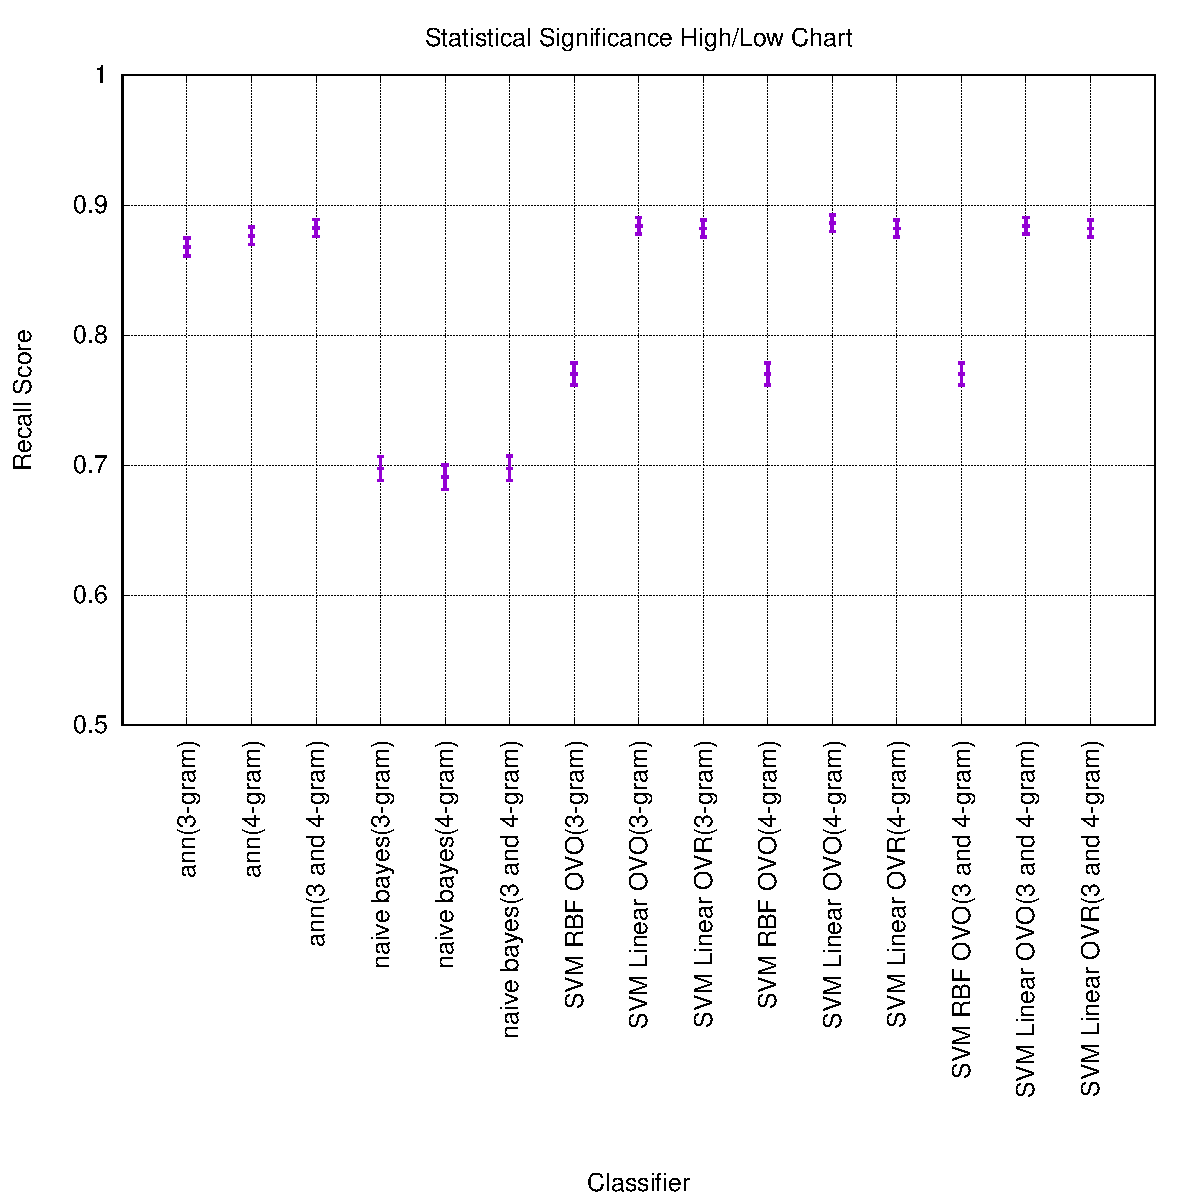
\includegraphics[width=.9\textwidth]{statsig_highlow.pdf}
  \caption{High/Low chart depicting the 95\% confidence interval for each
  classifier and feature representation combination implemented in this system.}
  \label{fig:stat_sig_highlow}
\end{figure*}

The statistical significance testing yields several insights into the
performance of the system. The clearest takeaway from this analysis is that all
classification runs that used an ANN classifier are significantly better than
all classification runs that used a Na\"ive Bayes classifier. The 
\textit{Recall} score separation between the 95\% interval lower bound of the
worst ANN performer and the upper bound of the best Na\"ive Bayes performer is
$0.154$, whereas the separation between the upper bound of the worst
ANN performer and the lower bound of the best ANN performer is merely $0.001$.
\par

Among the ANN classifiers, only the comparison between the ``ANN 3-gram'' and
``ANN 3 and 4-gram'' classification runs rejects the statistical null hypothesis
$H_0: \hat{r}_0 = \hat{r}_1$ since the upper bound of the 95\% confidence
interval of ``ANN 3-gram'' ($0.875$) is below the lower bound of the confidence
interval of ``ANN 3 and 4-gram'' ($0.876$), thus accepting the statistical
alternative hypothesis $H_a: \hat{r}_0 \neq \hat{r}_1$.\par

Comparing the ANN classifier with the variety of SVM classifier configurations
yields more interesting results, however. Several of the SVM variations either
matched or slightly out-performed the best ANN classifier. It is also
interesting to see that SVM classifiers using a Radial Basis Function (RBF)
kernel actually performed significantly worse when compared against their Linear
kernel counterparts. Another interesting insight into the SVM classification
runs is that feature representation did not have as profound an impact as it
did with either ANN or Na\"ive Bayes. Based on the 95\% confidence intervals,
there is no significant difference between any of the SVM Linear kernel
classifiers and the best non-SVM classifier (ANN using ``3 and 4-gram''
feature representation).\par

\section{Work Distribution}\label{sec:plan_roles}
The proof-of-concept implementation exercise is divided into seven (7)
primary task areas. The order in which the tasks are presented in this paper
does not necessarily represent the chronological order in which the tasks were
be carried out.

\subsection{Data Set Labeling}\label{sec:labeling_task}
As stated in Section \ref{subsec:eval_dataset}, the source data set for this
proof-of-concept needed to be refined in order to accommodate the
classification taxonomy as described in Section \ref{sec:design}. Although all
team members contributed to this task, \textbf{Mr. Marc Mailloux} serves as the
task's point of contact.

\subsection{Text Tokenization}\label{sec:tokenization_task}
Transforming the training and test sets from plain English into a form that 
ignores small derivations from the contextual meaning can improve the accuracy
of the model. For this task, \textbf{Mr. Marc Mailloux} serves as both the primary 
developer and the point of contact. 

\subsection{Text Embedding}\label{sec:embedding_task}
Transforming the text representation from plain English text to vector embeddings
which will be fed into the system. For this task, \textbf{Mr. Maxim Shelopugin} 
provides the main methodology and \textbf{Mr. Rolando Nieves} increases the 
performance for the multi-threaded environment.

\subsection{Cross-Validation}\label{sec:validation_task}
Separating the data set into training and testing, as well as providing
minor optimizations like double-counting is done in a separate module, and the
point of contact for it is \textbf{Mr. Maxim Shelopugin}. 

\subsection{Classifiers}\label{sec:classifier_task}
The classifier task, given its wide breadth, is divided among all team
members. A list of the classifiers that will be used, along with a short
explanation justifying their use, as well as the classifier's implementation
point of contact, follows:
\begin{itemize}
  \item Artificial Neuron Network (ANN) - ANNs possibly represent
  the most flexible of classifiers, both in the form of input they accept as
  well as the output they produce. The point of contact for this classifier is
  \textbf{Mr. Rolando Nieves}.
  \item Support Vector Machines (SVM) - SVMs have the possibility of requiring
  the least amount of computing power during both training (as compared with
  ANNs) and classification. The point of contact for this classifier will be
  \textbf{Mr. Marc Mailloux}.
  \item Na\"{i}ve Bayes - This was the classifier used in the \textit{Anti-Bully}
  system this proof-of-concept will be based on. It will be interesting to
  assess the impact, if any, of implementing the same classifier on a
  multi-class environment. The point of contact for this classifier will be
  \textbf{Mr. Maxim Shelopugin}.
\end{itemize}

The statistical significance testing, as described in Section
\ref{sec:evaluation}, will be implemented by \textbf{Mr. Rolando Nieves}. Mr.
Nieves will also serve as the point of contact for the classifier task.

\subsection{Presentation}\label{sec:presentation_task}
\textbf{Mr. Maxim Shelopugin} will be responsible for producing any materials
required to present the results of this proof-of-concept to interested parties,
including a summary poster.

\subsection{Final Report}\label{sec:report_task}
Although all team members will contribute content to it,
\textbf{Mr. Rolando Nieves} will be responsible for producing the final report
that will document the results observed while exercising the proof-of-concept
implementation documented in this paper.

\section{Conclusion}\label{sec:conclusion}

The proof-of-concept system documented in this report has proven to be a solid
enhancement of the efforts started by Michelle Li \cite{Li2016}. The system
provides good evidence that well-established machine learning techniques can
serve the greater good in helping address and possibly curb society's darker
impulses.

In current society, however, fielding such a system would levy more than just
technological challenges. Privacy concerns are a very important consideration
when putting the technology demonstrated in this report to practice. In the
opinion of the authors, some deployment choices could steer clear from such
privacy concerns, such as giving service users the option to deploy and activate
the system's features on their end, vs. forcing the deployment across the
entire service's installation base.

There are still areas where a system like the one documented in this report
could be improved upon. First among them is refining the algorithms such that
anomalies as those documented in Section \ref{subsec:ann_discussion} are better
mitigated. Agrawal et. al. \cite{agrawal2018deep} addresses one of the
enhancement suggestions, which is the portability of a trained system across
multiple communication platforms. Another opportunity for improvement lies in
enhancing the system such that either unsupervised learning or Reinforcement
Learning can replace the use of labeled data sets in what has been up to this
point a supervised learning system. Unsupervised learning would require
engineering the feature representation of text units such that patterns emerge
``organically.'' Reinforcement learning would require an automated reward system
that encourages the proper labeling of text units. Both of those endeavors have
the clear potential of proving very rewarding to any interested researchers.

\bibliographystyle{ieeetr}
\bibliography{final_report}


\end{document}
